\documentclass[bsc,frontabs,twoside,singlespacing,parskip,deptreport]{infthesis}
\usepackage{url}
\usepackage{amsmath}
\usepackage{xcolor}
\usepackage{listings}
\lstset{
  breaklines=true,
  postbreak=\mbox{\textcolor{red}{$\hookrightarrow$}\space},
}
\begin{document}

\title{This is the Project Title}

\author{Your Name}

\course{Master of Informatics}
\project{{\bf MInf Project (Part 1) Report}}

\date{\today}

\abstract{
This is an example of {\tt infthesis} style.
The file {\tt skeleton.tex} generates this document and can be 
used to get a ``skeleton'' for your thesis.
The abstract should summarise your report and fit in the space on the 
first page.
%
You may, of course, use any other software to write your report,
as long as you follow the same style. That means: producing a title
page as given here, and including a table of contents and bibliography.
}

\maketitle

\section*{Acknowledgements}
Acknowledgements go here. 

\tableofcontents

%\pagenumbering{arabic}


\chapter{Introduction}

The document structure should include:
\begin{itemize}
\item
The title page  in the format used above.
\item
An optional acknowledgements page.
\item
The table of contents.
\item
The report text divided into chapters as appropriate.
\item
The bibliography.
\end{itemize}

Commands for generating the title page appear in the skeleton file and
are self explanatory.
The file also includes commands to choose your report type (project
report, thesis or dissertation) and degree.
These will be placed in the appropriate place in the title page. 

The default behaviour of the documentclass is to produce documents typeset in
12 point.  Regardless of the formatting system you use, 
it is recommended that you submit your thesis printed (or copied) 
double sided.

The report should be printed single-spaced.
It should be 30 to 60 pages long, and preferably no shorter than 20 pages.
Appendices are in addition to this and you should place detail
here which may be too much or not strictly necessary when reading the relevant section.

\section{Using Sections}

Divide your chapters into sub-parts as appropriate.

\section{Citations}

Note that citations 
%%(like \cite{P1} or \cite{P2})
can be generated using {\tt BibTeX} or by using the
{\tt thebibliography} environment. This makes sure that the
table of contents includes an entry for the bibliography.
Of course you may use any other method as well.

\section{Options}

There are various documentclass options, see the documentation.  Here we are
using an option ({\tt bsc} or {\tt minf}) to choose the degree type, plus:
\begin{itemize}
\item {\tt frontabs} (recommended) to put the abstract on the front page;
\item {\tt twoside} (recommended) to format for two-sided printing, with
  each chapter starting on a right-hand page;
\item {\tt singlespacing} (required) for single-spaced formating; and
\item {\tt parskip} (a matter of taste) which alters the paragraph formatting so that
paragraphs are separated by a vertical space, and there is no
indentation at the start of each paragraph.
\end{itemize}

\chapter{Introduction}
%TODO: expand
The \textit{Chatting about data} project aims to explore the potentials of using chatbot technologies to empower users by increasing their understanding of their own health through data. The project explores different areas of human health: sleep, mental health, and nutrition. The latter provides an interesting variety of challenges that have been explored in academic and clinical trials, but never for the purpose of a comprehensive, general purpose consumer application. This might be an explanation of why it’s still not common to discuss your dietary habits with your favourite personal assistant, regardless of how ubiquitous the technology has become in the last decade. But while the trend of consumer voice assistants has been developing products as all-round helpful tools, which do not specialise in any one task, the lack of a clear winner in the space of textual digital assistants has resulted in the proliferation of programs with smaller scope. Known as chatbots, they usually specialize in accomplishing a small set of specific tasks, akin to the app model of the early smartphone era, and are similarly distributed through a centralized platform. Which means food logging, a facet of the growing quantified self movement that has exploded with the smartphone, might well be suitable for the scope of operations of chatbots. And just as the smartphone has not completely solved food logging, with adoption still relatively low compared to tracking other vitals and abandonment being high, the relatively unexplored area of natural language assistants in the context of \textit{m-health} (mobile health) still presents several unsolved problems. \\
A nutritional assistant must contain two essential features: the storage of foods consumed by the user, and the retrieval of such information for the purposes of informing dietary choices. There is a large variation in how these two tasks are accomplished among various existing solutions, and the aim of our project is proposing an implementation that, using a Natural Language interface and the ubiquity and capabilities of modern messaging platforms, makes interactions easier and more engaging. \\
Automated food logging in most commercial solutions is predominantly text based, with the user typing in the name of what they had on the day, selecting the closest match from a database of foods and their nutritional value, and estimating the amount of portions they consumed. It has also become popular to add an option to scan the barcodes that are present on all commercial food packaging, linked to their database entries. Some experiments have been conducted to estimate calorie content through image recognition, but there are few commercial products available to the general public, and most experimental implementations require a marker for dimension, which is a significant detriment to usability. \\
We propose implementing a hybrid textual and photographic input food assistant, where portion size can be specified by typing in a quantity, or by characterizing consumption in comparison to previous meals. This eliminates the cognitive load of using a complicated interface or trying to remember precise portion sizes, and will initiate a first user reflection on how much they have been eating recently, rather than focusing on number of calories tracked, based on the belief that relative quantities and overall trends could be more useful than rigorous data collection for the purposes of maintaining long term engagement. \\
The harder problem is information retrieval, or rather how to extract value from the data and display it in a useful manner. The traditional techniques include calorie counting and breakdown of nutritional information based on macro and micro nutrients, usually shown as a table, a graph, or a progress bar. These strategies have been disputed by the nutrition community, and do not seem to be effective on the general public, resulting in poor engagement and little understanding of underlying dietary issues. \\
Our solution involves handcrafting a small set of simple heuristics to detect harmful dietary patterns, and initiate a conversation by highlighting the issue and giving some suggestions to the user. While this method is unsatisfactory and ``does not scale'' to deal with the whole gamut of possible dietary problems, there are so far no better solutions in the literature, and we hope having a natural language dialogue would be more accessible to a non-expert than having to interpret the traditional markers in other fitness apps. \\

We describe our process in creating the Healthbot chatbot on Facebook Messenger, from designing its functionality, to implementing its logic, and running a user evaluation to compare it to \textit{MyFitnessPal}, one of the most popular food logging consumer technology. We also explain the various challenges we have encountered during our implementation, and how they relate to the wider field of chatbot design, as well as the insight we gained from our participants. Chapter 2 provides some background information on the state of the fields of chatbot development and its relationship with the quantified self movement and nutrition tracking in particular. Chapter 3 describes the design and architecture of Healthbot, along with a review of features that we originally set to implement, and why it was impossible to complete them. Chapter 4 shows the steps we have taken to review the chatbot's functionality, both during development and after, describing our evaluation study and participants' responses. Chapter 5 elaborates on the results gathered from the survey and observation of how participants interacted with the prototype, and identifies future problems that will have to be tackled before distribution to the public.\\
Our contributions to the field are implementing and deploying the first integration of textual and photographic food logging in a chatbot interface, as well as a comparative experiment between the chatbot and traditional diet tracking app on subjects from a similar demographic group. Our chatbot is also the first to utilise relative units of measurment for capturing logs, a simplification that has been well received from testers and shows some promise for future implementations.

\chapter{Background}
\section{The chatbot revolution}
Much has been said about how the rapid reduction in cost of the semiconductor has changed the world in a significant way in the last 60 years. The rapid spread of inexpensive and energy efficient computers, networks, and storage facilities, has revolutionised the way we access information, exchange goods and services, and communicate with one another. The diffusion of the smartphone, specifically, has brought forth an explosion in the amount of information generated globally, with more than $\frac{2}{3}$ of the world population owning one \cite{wearesocial}. Adults in the United Kingdom spend an average of 2 hours per day interacting with their phones, browsing the web, using applications, generating tracking data, and chatting, the latter being one of the most popular applications, with 42\% of mobile users \cite{mobilesocial} being active on social media. The top downloaded messaging applications, as of January 2018, are \textit{Messenger} and \textit{WhatsApp} (1.3 billion active users each), both owned by \textit{Facebook}, and \textit{WeChat} (980 million), owned by China-based \textit{Tencent} \cite{mobilestatista}. \\
Besides keeping up with friends and professional contacts, business transactions are also conducted through chat, either arranging sale and delivery of goods, or for customer assistance, the former being much more prevalent in Asia, where most medium and large size companies, as well as some smaller ones, have a WeChat presence and conduct what is known as \textit{conversational commerce}. Increasingly, many of these transactions are being automated through the deployment of \textit{chatbots} (bots), an evolution of classic conversational interfaces that have become popular in the last decade for commercial and entertainment applications \cite{Dale2016}. The most popular bot platform outside China is Facebook Messenger, which introduced the functionality to developers in April 2016 \cite{Messenger2016}, and it has since taken off with more than 200,000 bots on the platform as of December 2017 \cite{Messenger2017}. The development of Voice Assistants such as Google Assistant, Siri, Cortana, Alexa, or open-sourced Mycroft, have also pushed the deployment and popularity of conversational interfaces, either through voice or textual input. But if the above mentioned technologies try to be a general purpose digital assistant, most chatbots are typically concerned with a smaller domain problem, such as booking flights, checking the status of a bus, or telling a simple story \cite{meisel}. \\
The recent uptick in chatbot usage can not be attributed only to marketing, but also to significant advances in Natural Language Processing (NLP) and Natural Language Understanding (NLU). 
While early chatbot implementations relied on simple pattern matching rules based on recognition of specific words (entity recognition) or parts-of-speech (POS tagging), most of today's chatbot frameworks can leverage large corpora to apply machine learning algorithms, such as Intent analysis. Conversation can follow a slot, or a flow model: the latter is a hardcoded scripted flow diagram that guides the user through a preset conversation; the former specifies ``slots'' that contain some data the developer is interested in, and the chatbot will use NLP techniques to fill the slots from conversations with the user. Responses are typically pre-written and matched to an intent, but advances in deep learning are opening up possibilities for generative models, which create the answer from scratch \cite{Gregori}. Particularly successful can be combinations of several approaches, such as Serban, 2017's use of reinforcement learning to combine the approach of a generative deep learning model and a template-based retrieval model \cite{Serban2017}. Critical to the success of the chatbot is a good context management system, to ensure that a multi-turn conversation doesn't feel disjointed, and that previously entered information remains available to the chatbot throughout the session. All of this functionality is implemented by a growing variety of open source and commercial tools available today \cite{JavierCouto}.\\
From a service provider's perspective, the potential of using a chatbot instead of a human to provide customer service or present content can be very appealing, offering the opportunity of automating repetitive tasks. A successful example of a chatbot deployed in a classroom setting is Georgia Tech's \textit{Jill Watson}, which complemented a team of Teaching Assistants to answer questions on a high traffic class forum \cite{Eicher2016}. But if chatbots can decrease the load for a smaller team, and improve customer experience by decreasing response times, they can also cause increases in customer dissatisfaction. In fact, conversational skills and friendliness are important elements when interacting with a customer service representative \cite{Kang2013}. Within these interactions, a particular emphasis on tone should be given \cite{morris1988many}, an aspect of conversation that until recently had not been developed in bots \cite{Hu2018}. While a complete replacement is still far off, and would cause concern for the livelihood of a still large number of people, chatbots are likely to soon be adopted by more companies to deal with clients' initial queries, while having a human agent supervise the conversation and be ready to intervene when necessary. The centralization of services under a single interface might also address the phenomenon of ``app fatigue'': smartphone owners are no longer installing new apps, and when they do retention rates are abysmal \cite{appfatigue}. While giving up apps for chatbots might limit some kinds of deeper integration into users' devices, it also significantly increases the company's reach to everyone who is registered on a messaging platform, rather than the few who will choose to install new software. \\ 
Chatbot users report their main motivation to be the increase in productivity in information retrieval tasks, compared to installing an app, scanning a long webpage, or placing a phone call, as well as the possibility of receiving customised replies based on their own preferences \cite{10.1007/978-3-319-70284-1_30}. The decrease in attention spans in younger generations \cite{Wilmer2017} and addictive design might explain why young users of social media crave immediate feedback \cite{brandtzaeg2016should}. Thus, as a synchronous form of communication, chat might be perceived to increase productivity over an asynchronous medium like email, and is reflected in users' favouring conciseness in the chatbot's personality \cite{10.1007/978-3-319-67744-6_28}. Other reasons for people to use chatbots, to a lesser extent, are the entertainment value, the social aspect of conversation, and the novelty value, with users actively selecting chatbots as a tool because they fulfil some form of psychological gratification, according to the use and gratification theory \cite{10.1007/978-3-319-70284-1_30}. \\
Given the need of chatbots to be used productively, user needs will cause significant consequences for the field of Human-Computer Interaction (HCI): new paradigms of interface design will have to be invented, and novel approaches to combine different types of outputs will be possible \cite{Følstad2017}. Undoubtedly, conversational interfaces provide a great advantage to the less tech-savy, who might have trouble understanding the user interfaces of many bespoke applications, but will already be familiar to the ``unifying'' chat window, a philosophy promoted as Zero UI \cite{zeroui}. The blank canvas offered by the chat interface offers an unlimited potential for User Interface Design, to the point that, if the chatbot application is aware of enough information about its users, it might be able to create personalised interaction taylored to their preferences. Doing so may alleviate the growing digital divide that some segments of the population experience, because of the implicit biases of tech companies employees when designing user experience without considering the tech-illiterate \cite{Brandtzaeg2011}.
\section{Advances in mHealth}
Since the earliest days of chatbots, such as Eliza, which was modelled after a Rogerian psychotherapist \cite{weizenbaum1966eliza}, it is clear that conversational agents can have significant impact on health. Their applications, however, remained limited, for once because of the restriction of having to use a teletype, but mostly because the still primitive state of the technology made freeform chatting, and, crucially, the ability to understand anything about mental health, impossible. More recently, the development of cheap sensors and widespread connectivity through smartphones has spurned a growing sector of m-health applications. From the 2000s, mobile phone use made patient - doctor communication quicker and more frequent, as well as enabling some initial forms of monitoring and providing a hub for Body Area Network, including different medical sensors \cite{Patrick2008}. The 2010s have seen further developments along these uses, as well as the advance of "Artificial Intelligent" applications, provided by vast quantities of data collected through mobile devices, as well as advances of other Computer Science and Engineering disciplines, such as image recognition, virtual reality, robotics, drones, 3D-printing, and the Internet of Things (IoT) being applied to the medical field \cite{Pistorius2017}. The vast quantities of data being collected have helped to advance the state of the art on several medicinal application - but they also provide a valuable monetisable resource, both from the perspective of Big Data analysis, and for the number of for-profit advertising companies that will sell medical information to marketers and insurance companies \cite{tanner2016}. And whenever personal data is put online, it will also attract hackers, who might be interested in patient data for its resale value on the black market and for identity theft \cite{hackercare}. The sensitive nature of this kind of information makes it difficult to operate without breaking patient confidentiality, since anonymised medical records can be re-identified by correlating with outside sources \cite{Sweeney2001}, and even large experienced medical institution and data collection companies can breach existing regulations \cite{deepmindnhs}. \\
Smartphone and wearable devices users have also been collecting their own personal information, giving birth to the idea of the Quantified Self, or Personal Informatics. \cite{rapp20014}
Much of the Quantified Self movement is based on the idea that the automation of data gathering will lead into greater insight and improve our own health and behaviours by making us reflect and evaluate our past experiences. Data collection for Quantified Self purposes in activity and sleep tracking has boomed in the last decade, with the proliferation of inexpensive inertial measurement units and heartrate monitor sensors combined in wristworn factors, as well as step counting applications being bundled in many smartphones \cite{Crawford2015}.
Rivera and Pelayo, 2012 \cite{Rivera-Pelayo2012} propose a framework necessary for a self tracking app, based on the three activities of tracking cues, triggering and recall.
Tracking can be done through software logging or hardware sensors. Triggering can be active, when the user is prompted to reflect in a suitable context, or passive, where the information is simply displayed in a location the user can observe and notice significant changes. Recalling can be aided through different techniques, which usually involve a considerable amount of post-processing and enhanced by access to large datasets. There is still much work that could be done in the area of contextualization, by associating the collected data with other sources, and data fusion, comparing your own data with independent self or peer reporting, as well as better data visualization in attractive and intuitive ways. \\
One example where the quantified self phenomenon can have a real impact is preventive medicine, promoting healthy lifestyle to alleviate future medical issues. Diet, in particular, has been shown to benefit from open ended food-logging more than other methodologies \cite{Bingham1994}. While Turner-McGrievy, 2013 \cite{Turner-McGrievy2013} found little advantage in replacing a paper diet tracking system with a mobile application, Personal Activity trackers in their study did receive an advantage; this leads to speculation that the lack of improvement in the first group might have been caused by the diet tracker's UX. In fact, using the My Meal Mate app over a 6-month trial, Carter, 2013 \cite{carter2013adherence} reported increased adherence, usage, convenience, social usability, and overall satisfaction compared to traditional diet tracking. \\
Good examples of currently active commercial quantified self apps for fitness and nutrition are MyFitnessPal \cite{mfpwebsite} and Google Fit \cite{googlefitwebsite}, whose designs have been shown \cite{Suzianti2017} to prioritize continuance intention (the willingness to continue using the app), usability qualities (directness, informativeness, learnability, efficiency and simplicity), and user value features (satisfaction, customer need, attachment, pleasure and sociability). The usability of these interfaces, which include both a textual input and a barcode scanner for commercial products, has increased the number of DIY food loggers \cite{Alonso2015}; however, there is still some friction to a seamless logging experience \cite{Boushey2016}. The output of fitness tracking app is also of questionable usefulness: using calories as a primary metric is an oversimplification, as different kind of foods provide more nutritional value for the same caloric amount \cite{webmdcalories}. This might mislead a user in consuming more food than they should be, just to hit their calorie goal, or to leave some essential nutrient off their table, which can have negative consequence on overall health and impact their weight goals. In fact, Hebden, 2014 \cite{hebden2014} reports that user engagement with mHealth food logging solutions tapered off after a month of sustained use. Within the study, patients were most engaged by the text messaging component of the food logging system: this suggests that some of the issues with current interfaces might be alleviated by the use of a chatbot. \\
Chatbots have been speculated to provide a useful tool as a behavioural intervention technology, used to complement human practitioners in reaching a larger number of users and automate personalised messages \cite{Gabrielli2017}. Experimental and clinical trials using simpler informational chatbots have been made in various medical fields, such as counselling \cite{Cameron}, mental health intervention \cite{Elmasri2012} and sexual health information \cite{Brixey2017}, generally providing positive results, or at least giving indication that the medium might be used to address the specific issues.
Among the more successful experiments in Behavioural Health Intervention, the MobileCoach open source platform \cite{mobilecoacheu} was originally designed as a text messaging based system, which did some parsing on the backend but mostly relied on practitioner's interventions. It has now been redesigned as a full fledged online chat platform, which was perceived positively in clinical trials where participants treated for obesity interacted with a chatbot that exhibited a distinct personality \cite{Kowatsch2017}. \\
One successful attempt at making a dietary tracking chatbot is Forksy \cite{forksywebsite}, which seems to be still actively developed, but there are no statistics on its usage and success rates. From direct experience, Forksy is very aggressive with its reminder to log your meals, and does a nice job displaying your diary, but seems to have no ``smart'' features, and is inconsistent with the quality of its parsing.
\section{Making a smart chatbot application}
As researchers in many other fields in Computer Science are realising in the last decade, the collection of large quantities of data can have other uses besides record keeping, by leveraging the booming fields of machine learning and data science. This could eventually lead to make a truly useful chatbot, which in the future could replace or complement professional dietitians in a larger measure than today's solutions. \\
Ever since Richards, 1902 \cite{Richards1902a}, attempts have been made to algorithmically use food composition values to maximise food value per money spent. However, as Richards herself notes, "we know too little of the effect on digestibility, of cooking, and of the combination of two or more foods in one dish, or at one meal, to permit of very close calculation". \\
Even a century later, nutritional science still struggles to establish criteria to categorise individual food as ``good'' or ``bad'', because of the large number of nutrients each is made up of \cite{USDAFoodandNutritionService2007}. While dietary guidelines exist based on nutrients rather than foods, they often fail to be effective, because of the difficulty for consumers to find options that combine all nutritional recommendation, while also being economically accessible, convenient, and conforming to their taste and cultural preferences \cite{Green2015}. \\
To achieve a truly smart dietary assistant, given a vast amount of information about users, their habits and goals, we should be able to recommend an effective strategy to achieve the latter by analysing their choices in the former. As Gregori, 2017 \cite{Gregori} describes, the architecture of a chatbot requires four components: a frontend, a knowledge base, a backend and a corpus. While there are many tools that can be used for chatbot frontend and backend, finding an appropriate corpus and generating a knowledge base are domain specific tasks, with far less options available. \\
Even for a restricted dietary task such as reducing fats consumption, current expert systems are based off a set of handcrafted rules \cite{Prochaska2005}. While the medical community has made efforts to solidify their field into knowledge bases, there are no prevailing standards to read and interpret them, and although some attempts have been made to use knowledge graph representation to power a symptoms identifier chatbot \cite{minutoloa2017conversational}, there doesn't seem to be a canonical dietary knowledge base. Current commercial apps use a combined approach of total calorie counts and macro/micro nutrient percentages, but this is often insufficient to initiate healthy behaviours \cite{Davis2016}. \\
Despite the criticism for the occasional sensationalism, the emerging field of dietary epidemiology advocates a holistic approach to nutrition studies, by taking into account genetic, lifestyle and metabolic information as much as dietary records, making the mere tracking insufficient to draw anything but the most casual inferences on the users' health \cite{byers2001food}. But until this branch of the field develops enough to provide us with effective personalised nutrition (some recent startups would like us to believe that's already the case \cite{habitwebsite}), it's possible to use a more restricted approach based on recognising unbalanced diets from the lack or excess of certain key nutrients, abstracting the mechanics of quantifying exact measures from the users by providing more immediate advice through food recommendation. Data analysis techniques on food composition can be used to draw networks of complementary foods (foods that together fulfil nutritional needs) \cite{Kim2015a}, which could be used to give suggestions based on what users have already eaten. There are plenty of choices for nutritional value composition datasets (the most popular compiled from the United States Department of Agriculture \cite{usda}), and free or commercial APIs \cite{foodapis}.\\
%% social component
Success in activity tracking is influenced by demographics, with older and lower income subjects having lower rates of initial activation and retention \cite{Patel2017}. This problem may be caused by the bespoke user interface each fitness tracker comes with, which we believe a universal chat interface will alleviate. However, there are other factors worth considering for integration. \\
Popular fitness tracking apps often providing social networking functionalities, which have helped participants achieve their fitness goal through a combination of competition with their peers and social accountability \cite{chenchen2014}. Gamification has also proven useful \cite{doi:10.1001/jamainternmed.2017.3458}, and so have financial involvement, but only when profiled as a loss and not for modest gains \cite{doi:10.7326/M15-1635}. One company who successfully integrated diet tracking with all these aspects (gamification, monetary incentives and social accountability) was Gym-Pact (later Pact app), which rewarded users for tracking their calories, eating enough fruits and vegetables, and exercising, but took money from them if they didn't, and allowed users to post their progress to social media and compare it with their peers. The app reached a sufficiently large number of participants \cite{nudgingpracticioner} to sustain itself for several years, and a high percentage of users was frequently able to achieve their goals without cheating thanks to progress reviews from other users (but their business model was not profitable enough, and they closed in Summer 2017).
%% ease of use of image recognition
\section{Image recognition}
Most messaging apps today come with media functionality integrated; in particular, it's easy to take pictures and send them as a message from within the app itself. A diet tracking chatbot might benefit from the users' ability to take pictures and instantaneously receive feedback on their nutritional value. While, to the best of our knowledge, this has never been attempted within a chatbot interface, photographic diet diary have complemented food logging for many years, both in a traditional paper form to aid recollection \cite{Higgins2009}, and, more recently, electronically. For most of the photographic food logging app, portion size estimation requires placing a fiducial marker, an object with a distinctively recognisable pattern, in the frame of the image, to enable fitting a geometrical model on the entire picture \cite{Ahmad2016}. A slight twist on this has been given by Smartplate, a startup that uses a distinctively shaped plate to implement image based food tracking \cite{smartplate}.\\
A different approach was used by Google research with the Im2Calories Android app \cite{Myers2015}. Besides using a convolutional network based off a newly collected multilabel dataset to classify what the food in the picture is, different CNNs are also used to segment images and to estimate their 3D volumetry. This allows the app to assign calorie counts to images that contain different foods in the same plate, and to have more precise estimation of size. Unfortunately, neither the app nor the datasets have been publicly released. More recently, small startups like Calorie Mama\cite{caloriemamaai} and Bitesnap\cite{bitesnap}, as well as Samsung's digital assistant Bixby \cite{bixbyarticle}, have also implemented similar functionality, although it is still not clear how their models were trained or how effective they will be. \\
Among social media users, especially on the Instagram photo sharing platform, it's common to photograph images of aesthetically pleasing food. While this does by no mean provide an exhaustive nutritional history, it can be used as a further automation to save users from having to manually log their meals and extract nutritional information, as well as another potential avenue to establish social accountability to log healthy food \cite{Sharma:2015:MCN:2740908.2742754}. We will still have to use computer vision algorithms on this data, because Instagram tags are unreliable in identifying the content of the picture due to the large number of slang-related false positives \cite{hospedales2016}.
%% issues with image recognition????

\chapter{Implementation}
\section{Design}
As a dialogue agent, a chatbot needs to be designed with conversation with a human user in mind, each turn in the exchange supplying or retrieving information from the system.

To determine what kind of interactions the users and the chatbot should have, we started our design phase using the Botmock\footnote{botmock.com} tool to draft some conversation graphs. Botmock is a simple web application that allows its users to draw textboxes on a canvas and connect them to form a flow diagram, using a library of design elements that are adapted from popular chat interfaces, to give the impression that each box is part of a chatbot conversation.

\begin{figure}[h!]
  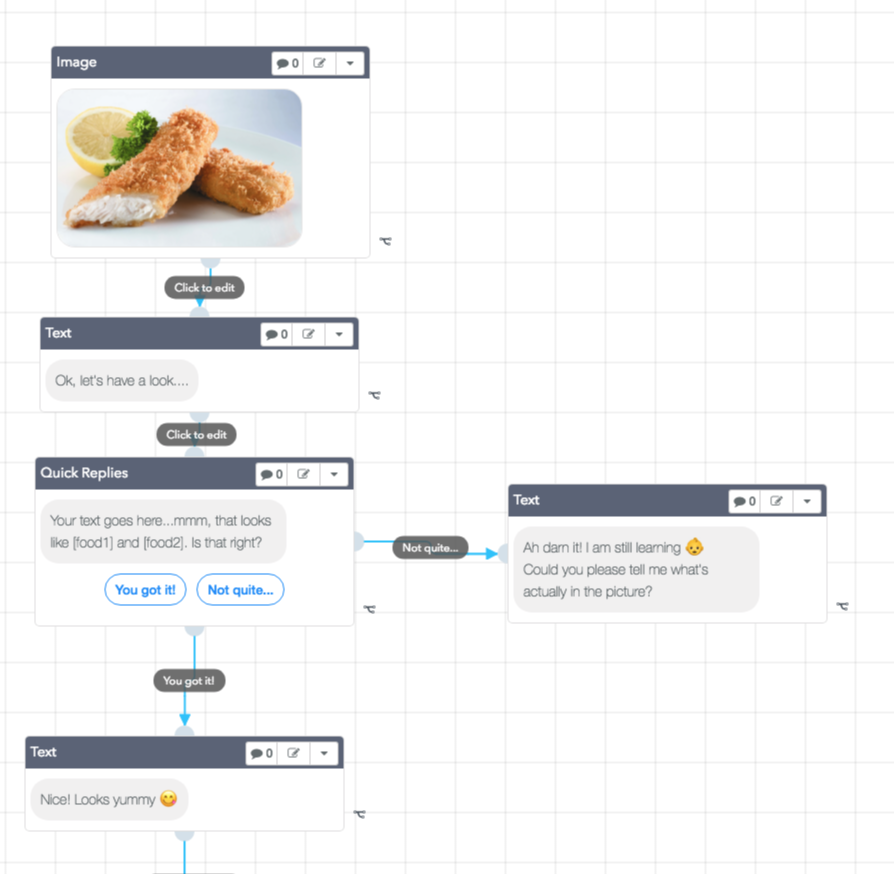
\includegraphics[width=\linewidth,keepaspectratio]{Botmock.png}
  \caption{An example conversation flow drafted in Botmock}
\end{figure}
One consideration when determining the tonality of our conversation sketches was determining what personality the chatbot should exhibit. Given the novelty of the medium in its modern form, we still lack comprehensive guidelines to craft what conversing with a bot should ``feel'' like, although as more chatbots are designed and deployed, some heuristics are beginning to emerge \cite{jessie}. Since chatbots users have shown to appreciate the fun aspect of designed chatbot personalities \cite{10.1007/978-3-319-67744-6_28}, we tried to imbue our conversations with some colloquial aspects, like using slang, calling the user names, and using emojis. \\
Additionally, we added some level or randomisation to the stock responses we would give, to make sure the chatbot did not feel repetitive, especially for frequent expressions. We also provided our bot with a cartoonish image of a robot (available on the internet under a free license) as a profile picture, and gave it the name \textit{Healthbot}, to give people an impression of talking with a real Facebook user.
\subsection{User functionality}
To establish a level of familiarity, rather than fetching a user's name from the client's account information, we initiate our first conversation by asking the user how they would like to be called. The rest of the introductory messages just describe the chatbot's functionalities.\\
Besides asking for help, users have three main available actions they can take: tell the chatbot what they are eating, send a picture of food, and ask the chatbot to recap what they had on a specific date. If the user doesn't specify a quantity or measurement to their meal, the chatbot will ask for details. To avoid bogging down the user with measuring their portions, and since we mostly want them to think about their diet in general terms, we encourage the use of relative rather than absolute quantities (\textit{more, less, same as usual}). We hope that using these measurements we will be able to maintain longer term user engagement, without sacrificing understanding of how much food is being consumed. Once we have this information, we send it through the Nutritionix API, to find out the nutritional content of that meal. \\
Sending a picture to the chatbot triggers a call to the \textit{clarifai} vision API, to understand what the contents of the image is, using their food model \cite{clarifaifood}. \textit{clarifai} returns a list of guesses for a picture, and their confidence value. If only one guess has confidence above the arbitrary threshold of 97\%, we save the food in the picture in our database; in any other case, we present the user with a list of the top three guesses as interactive buttons, so we can store the correct value in the database. 
\subsection{Nutritional analysis}
Once the user starts logging details about their food consumption, we will need to start analysing what they are eating to give them advice. Lacking comprehensive nutritional knowledge, the best we can do is crafting some elementary heuristics. 

The food retrieval intent queries the chatbot's database for all foods stored on a certain date. To aid user's reflection, we provide some basic data analysis, specifically on the food's quantity: 
\begin{itemize}
\item if there are more than 10 foods logged, with at least one having been consumed in large quantities and less than $\frac{2}{3}$ consumed in small quantities, we warn the user they might be overeating
\item if more than $\frac{2}{3}$ of a users' total logged foods on the day are smaller portions than usual, or if they have eaten less than 3 foods, we warn them about undereating. If they are asking for what they have eaten on the current date, they might just not have gotten around to log all their food yet; in that case, we send no warning if the time is before 10 PM
\end{itemize}

One example of food category that is often praised by dietitians for its high nutritional value \cite{bishoppgreens} is leafy green vegetables. To demonstrate the capabilities of chatbots as nutritional advisers, we handcrafted a list of leafy greens, which we try to match with every meal. If we do not observe the user eating any of these foods in 2 days, we prod them with a reminder. \\
Prodding in a chatbot context requires finding a very delicate balance: it can be too infrequent, making it less useful for users who are interested in being reminded; but if too frequent, it  might soon become annoying. For example, the Forksy nutritional chatbot \cite{forksywebsite} sends a reminder to record your food for every single meal (at least 3 a day). This causes the bot to feel overbearing, and it might actually drive the user away. Forksy's solution is asking the user what time they want to receive their next reminder; but if no food is logged, it gives no option to deactivate reminders completely, and keeps asking for meals every day of inactivity. \\
We attempted to solve this problem by staggering the no usage messages at increasing intervals, first after one day of inactivity, then on the second day, and after that the fourth, seventh and fifteenth, to maximise our chances of getting a forgetful user to start messaging again, without being too annoying if they choose not to. Larger amount of data analysis might be used in the future to determine when, based on current dietary habits or external inputs, the notification might be more effective in nudging the user into resuming logging or eating vegetables, and eventually provide an overall more active prompting system that takes into account correct dietary practices.

\section{Architecture}
Our chatbot's architecture is composed of a natural language interface in \textit{Google Dialogflow}, hooking up to an \textit{Express.js} server running a \textit{Heroku} instance, storing data on a hosted \textit{MongoDB}, and retrieving other information from external APIs. The agent itself is served as a bot on Facebook Messenger; while there are many possible integrations for Dialogflow, and we considered using \textit{Slack} as a distribution channel because of its first class support for bot users, eventually we chose Facebook for its popularity, as it allowed us to serve the bot to any of its billion users without them having to install any additional software.
\subsection{Dialogflow components}
There are several Natural Language Understanding platform specifically designed to create and deploy chatbots easily and quickly. Our choice fell on \textit{Google Dialogflow} (at the time \textit{API.AI}), because of its ease of integrations with most popular messaging platform, ease of development, responsiveness and solid NLP functionality. 

A Dialogflow agent is set up with a library of patterns, \textit{intents}, that use example sentences or templates to parse inputs to the chatbot. Templates include parameters whose types are called \textit{entities}, some of which are already defined by Dialogflow, but new ones can also be added by the programmer. One of the standout capabilities of Dialogflow is that a parameter can be marked as required by the intent, so if the initial utterance does not contain it, the chatbot will prompt the user to specify the new parameter. \\
To maintain the flow of conversation, an intent can be followed by another, based on what the user replies, with a context object which stores all parameters passed from the original intent down to all its followups. \\
Each intent can trigger an immediate response, as defined on the Dialogflow console, or it can trigger an \textit{Action} to be fulfilled by the \textit{Webhook}. \textit{Actions} are functions held on the server that can access the parameters of the current intent, execute their own logic, call external APIs etc. They usually are triggered as a POST request to the webhook's address, with the request JSON object as its body, and the HTTP response determines the behaviour of the chatbot, either by replying with more text, sending media or rich text, or triggering an \textit{event}, which executes an intent just as one of the triggering sentences had been sent by the user. \\
Small talk intents are also defined as part of Dialogflow to take care of common sentences unrelated to the chatbot's domain, and Dialogflow's machine learning engine can be interacted with through a Training console (still in Beta at the time of writing), which can be used to correct intent and parameter recognition (and indirectly, to gain insight into how the engine's model classifies new text).

Our chatbot defines the following intents:
\begin{itemize}
  \item \textit{First interaction} is the initial intent, triggered by the Facebook Messenger "Get Started" button or with the "Greetings" keyword for debugging purposes. This asks the user what their name is, and is followed up by 
  \begin{itemize}
  	\item \textit{Name save} which waits for a name to be given, and saves it to the database
        \item \textit{Name confirmed} replies with a welcome explanation message
  \end{itemize}
  \item \textit{Food log - text} is triggered when the user adds a meal to the log. It takes required parameters of food (as a list), quantities, and optional parameters of meal name and date
  \item \textit{Send food pic} waits for a Facebook Messenger Media object (a picture in our case) to trigger an action which runs image recognition. If no unique match is found, 
  \begin{itemize}
    \item \textit{Send food pic - no} is triggered by the webhook whenever there is no clear candidate for classification of a picture
    \item \textit{Clarify food pic} recognises user's sending a clarification for what the food was, through a Facebook Messenger button. To make sure the button's message matches this intent and not the generic food logging, a \textit{messenger\_button} token is appended to the message payload
  \end{itemize}
  \begin{itemize}
    \item \textit{Send food pic - yes} is launched whenever a picture is classified correctly, and just triggers the Analyse food pic intent
    \item \textit{Analyse food pic} takes the food content found in a picture received from the user, analyses and stores the result into a database
  \end{itemize}
  \item \textit{Help} matches a request for help with a few reminders of the chatbot's functionalities
  \item \textit{Date retrieval} is used to query for past food logs, taking just a date as a parameter. For logging purposes, with removal functionality to be implemented in the future,
  \begin{itemize}
        \item \textit{Date retrieval - false} will recognise when the user declares the food log for that day to be incorrect
  \end{itemize}
  \item \textit{What's my name} is mainly a debugging intent, to check if the chatbot has managed to successfully save the name for the current user in the database
  \item \textit{Sinkhole} is used for training purposes to redirect all the intents that were misclassified
\end{itemize}
Our chatbot defines the following entities:
\begin{itemize}
  \item \textit{meal} enumerates four different meals: breakfast, lunch, dinner and snacks
  \item \textit{quantity} contains a list of all the different measurement units for food
  \item \textit{meal-quantities} combines quantities with quantifiers (a, some, integers etc.)
  \item \textit{approximate-quantifier}
  \item \textit{date-ext} extends the \textit{@sys.date} object with today and tomorrow
\end{itemize}

\subsection{Backend}
By default, the Dialogflow interface includes a small inline editor to implement some simple webhook logic. While the web interface is limiting for creating a backend of the complexity required, it's easy to export this example code to \textit{Google Cloud Functions} \cite{gcfwebsite}, Google's serverless cloud function service, and their own database, storage and analytics tool, Firebase. \\
The sample code consists of an Express.js \cite{expresswebsite} web server, which listens to POST requests to the \textit{/webhook} route to the server, which will be sent from Dialogflow, and provides helper functions to craft the appropriate response as a JSON object, which will trigger a reply through the chat client. The largest portion of the code is the \textit{action-handlers} dictionary, which associates a different function to any of the Dialogflow intents. 

We started developing our webhook from this starting example in GCF, but we soon realised that a core requirement of our design, the ability to call up external APIs, was not possible under the free tier of Google Cloud. Thus, it was necessary to find a replacement. Some options that were considered were Apache OpenWhisk \footnote{https://openwhisk.apache.org}, Captain Duck Duck \footnote{https://github.com/githubsaturn/captainduckduck}, Amazon Web Service Lambda or Elastic Beanstalk \footnote{https://aws.amazon/com/products}, Dokku \footnote{https://github.com/dokku/dokku}, 1backend \footnote{https://github.com/1backend/1backend}. \\
In the end, Heroku \footnote{https://heroku.com} was selected as a solution because of its many productivity advantages. Among the many alternative the popular Platform as a Service (PaaS) solutions offer, we took into consideration the mature tooling, the easy to use deployment infrastructure, which consist of simply pushing the code to a version controlled repository, the automatic inclusion of a free domain name, and simple (but barebone) scheduling functionality. Heroku offers both a free and a paid tier; for our purposes of creating a prototype, the free tier offers all required functionality; however, it would not be sufficient to power a chatbot infrastructure in a production setting, as there are limits to free users' capabilities, most notably a temporary suspension (and extensive wake up times) after an hour of inactivity.

Having moved to a full PaaS implementation, we were able to expand our program from a single file to several modules, which was necessary to avoid a large unwieldy single file, and allows us to compartmentalize between different types of functionality.
\begin{itemize}
  \item \textit{index.js} is the main function for the Express server, it runs in a loop waiting to receive any requests, and serves a response for any predefined URLs. On a POST request to \textit{/webhook}, it will read the request body to find the action's name and parameters, and calls a function as defined in the \textit{actionHandlers} dictionary. Most intents match one-to-one to an inline function in this object, although some are defined in an external module
  \item \textit{messenger.js} contains output functions to send a reply to the user, either going through the Dialogflow API, or directly through the user's Facebook Messenger account (necessary for sending a message on a predetermined schedule, without a user initiating the conversation)
  \item \textit{picture.js} handles all intents related to pictures, from querying the \textit{clarifai} to handling incorrect or imprecise guesses.
  \item \textit{mongo.js} abstracts some of the low level database, like connecting to the database and querying the username
  \item \textit{analysis.js} deals with all food related activity, like querying the Nutritionix API and analyse users' dietary records
  \item \textit{strings.js} contains all messages the chatbot will send to the user, all collected in one file for ease of editing
  \item \textit{worker.js} defines a set of functions to run periodically, which will verify some information about each of the chatbot users, and send an appropriate message
\end{itemize}
The latter module, unlike all the others, does not export any of its functions, but runs every day at 8 AM GMT by the Heroku scheduler add-on.

We considered training our own food recognition model by training on the Food-101 dataset using the DeepFood Caffe model \cite{liu2016deepfood}, but after an initial evaluation it seemed ike precision would not be much better than \textit{clarifai}, so we opted to use the free service and save ourselves from training the model and store it on our server.
\subsubsection{Database}
When considering which database to use, the variety of offerings is truly staggering, so we decided to optimise for speed of development, by using a NoSQL database, which combines speed and scalability with the flexibility of not having to predefine a schema, an essential feature when building a prototype which has to undergo through several changes before finalising its design. While some chatbots designs integrate a graph database, which allows rapid aggregation over different entities, it was unnecessary for our current usagee, and we preferred to adopt a more widely used and better supported product.

Our final choice was a MongoDB database free instance hosted on \textit{mlab.com}. The database consist of a single collection, users, with a unique document for each user. \\
Besides containing identifying information such as a unique Dialogflow ID, a session ID to initiate messenger conversations and a name, we also store a list of \textit{meals}, which we defined as objects containing a list of food items, their quantities, a date, and an optional meal name (lunch, dinner, breakfast or snacks). \\
Finally, we have a \textit{counter} object, which stores values for the number of days since the user has logged any food, the number of days since the user has had any green leaf vegetables, and the total number of days. These are used to determine whether a reminder should be sent to that specific user about any of those issues (the total count reminder is used to ask for feedback about our experiment after three days, to collect some data while participants are still engaged with the chatbot).
\section{Roadblocks}
While we have developed and delivered a fully functional chatbot, there are many features that we would have liked to have but could not implement for lack of time. Other features were started, but could not be completed. \\
During our planning stage, for instance, we envisioned Healthbot to be able to answer some facts about the nutritional properties of any food the user would ask about, and to have the ability of adding recurring meals, so that if a user had a habit of having the same food every day they would not need to add it again and again. \\
We also started scripting some ``challenges'' the user could ask to be set, to improve their habits through gamifying the tracking activity; we explored options for both individual and group challenges.\\
Eventually, all of these projects had to be suspended because we had to prioritise the core features; for the other aspects listed below, we started working on an implementation, but encountered some obstacles.
\subsection{Instagram integration}
A unique feature of our initial chatbot design was its integration with \textit{Instagram}. If a user had an account on the social network, we would have asked them during the onboarding procedure to log into their account to generate a unique access key, which we would later have used to crawl their image history for food pictures.\\
We developed the onboarding dialogue sequence, giving the user a choice on whether to add an account or not, and we registered an Instagram developer account and an application to generate unique login URL. If a user logged in through this link, they would have been redirected to a custom address on our server where the access token would have been saved to their account.

We completed our implementation of this first phase, and successfully tested the token generation on our own account. But as we were developing the crawler implementation, our application was suspended for Terms of Service violation. Speaking in person with a Facebook engineer, they speculated that the reason for the ban was that the picture retrieval API is only intended for building alternative clients, making our idea infeasible. \\
In hindsight, it was for the better we stopped working on this feature: during the evaluation period, following the fallback from journalistic investigation over Facebook's excessively permissive data sharing practices \cite{cambridgeanalytica}, the Instagram API was completely deprecated \cite{instagramdeprecated}.

An alternative with a more permissive API is \textit{Flickr} \cite{flickr}, but we did not explore the possibility of using this smaller social network.
\subsection{Defining a food entity}
The Dialogflow predefined entities do not include one for food. This is in fact a nontrivial problem, because enumerating all possible food requires knowing about both ``raw'' ingredients, and commercial food which might be referred to as their brand name or with a specific product denomination. We therefore tried to handcraft our own food corpus, in the hope it would provide sufficient coverage.

To collect food entities, we first used the Open Food Facts database \cite{openfoodfacts}. Besides being freely accessible, this option was selected because of the large number of entries, $374,259$, the presence of generic food identifiers associated with commercial product for 59,383 of the entries, and a nutritional approved health rating on a A to F scale. Moreover, besides a raw data export, the service provides an experimental JSON API For online queries. \\
The raw database was exported as a MongoDB \cite{mongo} object, in \textit{bson} format. After having created an empty \textit{openfooddata} table, using the \textit{mongoimport} command we copy the contents of this object in the new database. Then, through the mongo console, we wrote a script to extract all food with a name in English.
\begin{lstlisting}
var cursor = db.products.find( 
    {$and: [
      {$or: [
           {``generic_name'' :  {$ne: "", '$exists':true}},
           {``generic_name_en'' :  {$ne: "", '$exists':true}}
        ]},
      {"countries" : {$regex: ``en|UK|United States|Canada''}
    ]}
)

var cursor = db.products.find({$and: [{$or: [{"" :  {$ne: ", '$exists':true}},{"generic_name_en": {$ne: ", '$exists':true}}]}, {"countries" : {$regex: ``en|UK|United States|Canada''}}]})
while (myCursor.hasNext()) {
   printjson(myCursor.next());
}
\end{lstlisting}

Unfortunately, this produced only 795 food item which were indexed as being listed in English, and had a proper name; manual testing for common foods resulted in several misses.\\
Subsequently, we found an online corpus of British raw food at LanguaL.org \cite{langual}(1316 items), but it was also insufficient for common queries. 

In the end, we decided to compromise, deeming missing on a less common food being logged more harmful than false positives. Our final approach was marking the food parameters as a \textit{@sys.any} entity, which is equivalent to a wildcard match. This is fine for a more structured intent, where the user prefaces tier logged food with an action verb (``I ate'', ``I had'' etc.), but these are not sufficient to capture the full range of inputs, as some user will also just say the name of the food. To catch those cases, we had to add an intent case which just matches entity \textit{@sys.any}, but that obviously has the unwanted consequence of also catching utterances that match neither the intent nor the smalltalk module.
\subsection{Classifying food}
Just like our handcrafted leafy green vegetable set, we would have liked the capability of automatically recognise whenever food belonged to a certain category (meat, fish, nuts etc.), which we would have used to create a set of simple heuristics to detect food missing from the user's diet. \\
The apparently simple task of associating the name of a food to a category is deceptively complex; even humans assign multiple categories to the same food (e.g. fruit or snack for \textit{apple}), and thinking about a certain food as belonging to a certain category will influence their beliefs in regard to its nutritional properties \cite{Hayes2011}.

Our naive attempt to classify food  according to its category was to cluster it based on its nutritional values: ideally, similar kind of foods would have ended up being classified in the same clusters ("high in sugar", "high in protein", "low in vitamins" etc.) and manual inspection of classified data could have been used to assign an intuitive category to each cluster. 

The \textit{k-means clustering} algorithm is used to group points in n-dimensional space into a predetermined $k$ clusters, by iteratively computing the cluster each point belongs to, based on a distance metric, until cluster membership becomes stable.\\
While our vector space was 250-dimensional, the number of distinct nutritional values identified by the USDA nutritional database, it is not trivial to determine the value of $k$. If we had had a distinctive number of food groups we wanted to obtain (like, for instance, the 10 categories identified by the Australian National Nutrition Survey of 1995 \cite{NNS1995}), we could have used that as $k$, but obviously any kind of foods that belonged to a cluster we have not considered would have been incorrectly classified. Napoleon (2011)\cite{napoleon} describes an algorithm to both automatically select a value $k$, and to reduce the dimensionality of our data set. This allows us to reduce computation, by eliminating nutrients that do not contribute significantly to the classification, and is a necessary operation, because the size of our training set was too small compared to the dimension of each data point. Known in the literature as \textit{curse of dimensionality}, it can lead to a variety of issues that would make any classification meaningless \cite{kriegel2009}.\\
Once clusterings for the training set were calculated, any subsequent food the user logged would have been classified based on its distance from the calculated cluster centres.

We built a training dataset by fetching from the Nutritionix API the nutritional values of the 1316 foods in the LanguaL.org dataset, minus the 213 foods Nutritionix had no nutritional value on record for. The Nutritionix API returns a list of values of type (ID, quantity), where the ID Corresponds to nutritional values as identified by USDA. Because the free tier of the API is rate-limited to 200 requests per day, we wrote a script to break up the dataset into smaller chunks, download a portion of data every day, and recombine it. Having collected all our samples, we passed the data to a custom Node script, using the \textit{mljs} library \footnote{https://github.com/mljs}, to expand each food's value into a 250-dimensional vector, and perform dimensionality reduction using PCA \cite{Ding2004}, find good starting cluster centres, and executes k-means clustering on the entire dataset using the \textit{clusterfck} library \footnote{https://github.com/tayden/clusterfck}. The cluster centres were then stored to a file, with the intention of them being read by the application for classifying new food. 

All attempts at classification, however, where disastrous. While we used the algorithm from Ding, 2004 \cite{Ding2004}, to dynamically identify the number of cluster centres with highest variance (a number of 7 for our dataset), our results were only marginally better than other clusterings. For any number of clusters we tried, most datapoints would group around 2 or 3 cluster centres, with one centre attracting around 800 values, a few hundreds for the other two, and all other centres having between 10 and no value. This result is corroborated by Kim et al. (2015)\cite{Kim2015a}'s finding that foods of similar origins do not necessary cluster together when grouping based on raw nutritional values. Their proposed network classification and metrics of nutritional fitness do offer a potential method to recommend complementary meals for the chatbot, but deriving the full network from the provided dataset would have required a significant amount of time, and each query would also require calculations that would take so long as to make a chatbot unresponsive.

Automatic classification of foods into distinct groups is still an open question. Besides nutrient counts, alternative classification methods could be usage of word embeddings in recipes \cite{food2vec}. While this might be a good way to find if two foods are culinarily related, it does not necessarily satisfy the property of nutritional equivalence, which is what we would ultimately like Healthbot to do.
Eftimov, 2017 \cite{Eftimov2017} developed an automatic classification method for European standard food classification system FoodEx2, which lists not only composition values, but also chemical contaminants, food consumption and pesticide residuals. Their algorithm goes through a classified learning phase and a probabilistic natural language extraction phase for description, which achieves a good accuracy of 89\%, but the resulting classification categories are too broad to be useful for our purposes.


%Expert system in \cite{Chen2012} define nutritional rules as: 
%Underweight
%Overweight
%Mild Obesity
%Moderate Obesity
%Severe Obesity
%Morbid Obesity
%Abdominal Obesity
%Excessive Percentage of body fat
%Significant weight loss
%Severe weight loss
%Mild PEM
%Moderate PEM
%Severe PEM
%Kwashiorkor
%Marasmus
%Excessive caloric intake
%Adequate caloric intake
%Inadequate caloric intake
%Extreme energy restriction
%Excessive carbohydrate intake
%Inadequate carbohydrate intake
%Excessive sugar intake
%Excessive total fat intake
%Inadequate total fat intake
%Excessive protein intake
%Inadequate protein intake
%Excessive dietary fiber intake
%Inadequate dietary fiber intake
%Excessive cholesterol intake
%Excessive sodium intake
%Excessive mineral intake
%Inadequate mineral intake
%Excessive Vitamin Intake
%Inadequate Vitamin Intake
%Excessive Fluid Intake
%Inadequate Fluid Intake
%PEM for HD\&PD
%Inadequate caloric intake - HD\&PD
%Excessive protein intake – Chronic Renal Failure
%Inadequate protein intake – HD\&PD)
%Inadequate HBV protein intake – Renal Disease
%Excessive sodium intake – Renal Disease
%Excessive phosphate intake – HD\&PD
%Excessive potassium intake – HD\&PD
%Excessive water intake – HD
%Excessive SFA intake – hyperlipidemia

\chapter{Evaluation}
As with all software artefacts that have a user facing component, testing can be lead both on a technical level and on a usability level. Since the chatbot infrastructure contains many different components, it will be necessary to conduct some testing on the robustness of each.
\section{Testing}
Throughout the whole implementation, particular care was taken to follow software engineering best practices. Because JavaScript is a dynamically typed language, we lack a compiler's check for code correctness. As a consequence, we have to run code to find out if it works. To avoid deploying a broken commit to the server, we wrote a git pre-commit hook to test if the program doesn't crash immediately, and to pass a linter to catch any syntax error in the code:
\begin{lstlisting}
npm start > /dev/null &
sleep 5
if ``eslint *.js`` && [[ -n `pidof -k node` ]] ; then
    echo "Pass linter and npm doesn't crash"
    exit 0
else
    pkill node
    exit 1
fi
\end{lstlisting}
While this was a good tool to statically catch errors, some bugs would only emerge through dynamic testing. While the \textit{testmybot} unit test library \cite{} looked like a promising solution for establishing a routine of test-driven development, it soon was evident that the Facebook hooks for the underlying Botium library \cite{} are still not mature enough to be used in production. Therefore, rather than having a collection of sample conversations we could feed \textit{testmybot} to determine whether any new code change would break any of the responses we had been getting before, we had to resort to manually testing each new feature, by messaging the chatbot from a personal Facebook account, repeating the same script for each different functionality we had previously implemented. Most debugging information was printed to the Heroku server logs through the \textit{console.log} JavaScript function.
\section{Evaluation}
For our evaluation, we ran an experiment giving out the chatbot to 11 university students, all within ages of 20 to 25 and at least moderately physically active, to use for a week. As a control group, another 9 university students were prescribed to use the MyFitnessPal app for the same duration. All users were recruited through Facebook chat or in person, and all were given the OK to start the evaluation on the same day after having read and signed a consent form describing the experiment and the tester's role in it. In retrospect, having a more gradual rollout might have helped with spotting the first bugs sooner, and giving us a chance to fix the underlying issues without compromising the platform for every other user. As it was, while we identified several issues and features that would have been immediately easy to add, we did not push most of the modification to avoid breaking existing users' workflows. Unfortunately Facebook does not allow to have a separate testing and production environments until the application goes through a first review process, which we couldn't afford to spend time going through.
\subsection{Record keeping}
Since this was our first usage of the chatbot outside our own testing, we expected to encounter a variety of bugs and phrasings that it had never encountered from us. We set up a detailed logging function for all error case, printing the user ID as well so as to be able to reconstruct the causes at a later stage. We could also access a complete record of all communication through the Facebook app console, as well as having a list of intents identified and how the parameters were matched from the Dialogflow agent. While having this much access gave us some great insight into what might be affecting faulty behaviours, it was also concerning how we could read the conversations in their entirety, and while Dialogflow allows to deactivate the logging, there was no way of doing that through Facebook. And even if there was, it would be trivially easy to still log everything through the server.


\subsection{Experiment description - survey, in person interview}
To initiate the experiment, the chatbot users' Facebook profiles were added as testers through the Facebook developer console. They were then sent a link to the chatbot's Facebook page, where they could press a clearly visible button to start chatting. This would open a chat window, where they had the option of pressing a button to get started before being taken through their first conversation. Users were given no indication on how to precede, except for the chatbot's introductory message. Over the course of the evaluation, users sent us some questions (never through the chatbot) on what they could do with it. \\
The MyFitnessPal testers were asked to give feedback a week after the evaluation started; the bot testers were sent feedback forms after 9 days.
The surveys sent to both testers were built using the Google Forms online tool. Most questions were similar to both questionnaires, with some variation when it came to input methods and displays dependent on the app. In compliance with the consent form, none of the questions were made compulsory, and the survey was made anonymous.
The questionnaire asked some background information on the participant, to establish levels of fitness and computer literacy, thoughts on nutrition and previous dietary and food tracking histories.
Testers were then asked their opinion on the usability, utility, pleasantness of the entire platform they were evaluating, as well as for each specific functionality, and if they had any feedback on things they would have liked to see. Some answers were multiple choices, checkboxes or Likert scales, but most were open text input to allow the participant to give a full explanation of the reasoning behind their answer
\subsubsection{Survey Response}
7 participants responded to the My Fitness Pal survey within the first day, and 9 to the chatbot specific survey. While some questions were answered by all the participants who took the survey, none of the open ended questions were answered by all, sometimes with around half the respondents ignoring one question (??Verify??). \\
Participants seemed to be distributed similarly across the two trials, with chatbot users being slightly more proficient with computers, as well as being more aware of their fitness levels. Similar splits were evident in the proportions of participants who had died before, with around three quarters of participants citing a good current health or scepticism with established diet, and some chatbot users using laziness as a motivation. The minority of users who had dieted chose to do so because of environmental, athletic or health-related issues, but did not maintain dieting after reaching their goals, or because of commitment issues. Among both groups, about half the participants consistently had 3 meals per day, with some having a variable number of meals and no participants consuming less than two; our chatbot users however in general snacked less than My Fitness Pal users (there's a possibility that these answers might have been influenced by the experiment, even if participants were encouraged to think about their behaviour before; the fact that My Fitness Pal presents snack as a distinctly separate category, and the chatbot doesn't, might have affected responses to this question). \\
About half of the participants reported having tracked their diet before, either keeping a food diary, memorizing their meal, or, the majority of respondents, using My Fitness Pal, and the majority of previous trackers also kept a record of their snacks. \\
For unclear reasons, more than half the respondents skipped the section about their dietary makeup, but for who did fill it in, definitions of ``balanced diet'' varied significantly: while a majority named a variation of having a correct proportion of Protein, Carbohydrates and Fats, with some allowing for vitamins and minerals as well, others named calories as a main concern, reducing some unhealthy food groups and increasing others, or avoiding stressing about their diet and making sure to have what made them feel good. Only half of the respondents consider their diet to be balanced, including all those who planned their meals in advanced, and most respondents tend to cook their own meals, eat out or do both things in equal measure. \\
My Fitness Pal user found the app on average more useful than chatbot user, although the latter was rated as generally more pleasant to use. The food diary, the macronutrient breakdown graph and the remaining calorie counter were all generally considered clear and useful, with the graph being the most pleasant feedback. For input, the majority of users preferred scanning the barcode of the meal they were having, although for some the kind of food they were eating was a factor, and people who tended to cook their own food preferred text entries. All users had some issues with finding the food they wanted using text entry, but no one complained about the method being too slow; barcode scanning seemed to perform better, with only some users reporting difficulties identifying a barcode or matching the correct item in the database. By contrast, chatbot users generally found the feedback useless, or insufficient. Chatting was highly preferred as an input method, although several participants didn't find it understood their queries well enough, and some were annoyed by the prompts for size. Some users who took pictures for input found it wasn't accurate, but the larger problem for the feature seemed to be people who weren't aware of the functionality. \\
Retention rates were much higher for My Fitness Pal users, with the largest missed meals estimated to be 5, and some user logging all their meals; chatbot users, instead, were much less active, with one person logging almost every meal, and everyone else estimating having missed between 5 and 20. In both cases, the leading cause of missing a meal log was lack of time or forgetfulness, with some chatbot users finding input methods cumbersome or lack of interest because the feedback didn't seem useful. As a consequence, almost all chatbot testers did not log their meals on several days. Half of the users report having received a reminder the day after, with the other saying they didn't (which might be explainable by the fact that, while everyone received a reminder, it wasn't necessarily after a day of inactivity). The reminders were generally found to be useful, and mostly made the users log their food on the day, and one user even expressed a desire to receive more frequent prompts to avoid forgetting more meals. My Fitness Pal also provided a reminder functionality, but it's off by default. All users who turned it on got a reminder, but it didn't make them use the app after. \\
One stark difference in response between chatbot and app user was on preference between noting their food records with absolute measurement (number of portions or unit of measurement plus numerical value). My Fitness Pal users overwhelmingly declared a preference for absolute value metrics, because of the need to calculate precise calorie counts that the app provides, and as a more reliable comparison method to standard recommended portion sizes. The majority of chatbot users instead indicated a preference for relative values, because it's easier not to have to constantly measure portions. \\
Despite the fact that the utility of a food diary comes from the ability to look back on previous meals, only a third of the chatbot users, and just over half the app users took advantage of this feature at a later date, and those who did reported the information presented to them to be accurate, but unhelpful; in fact, about half of the chatbot users and two thirds of the app user don't think using the meal log has given them a better idea of how they eat. \\
Overall, most participants did not think that logging their food had helped them to eat better, although for many users that was because they already are happy with their diet. Those that registered a positive impact mentioned that having a better oversight on their food trends did prove helpful for them, and My Fitness Pal user specified sugar tracking and suggested recipes as useful features, although some comments also pointed out that the paid version of the app could have been more useful. However, $\frac{2}{3}$ of chatbot users found that they had become more ``mindful'' about their diet by using the chatbot, as opposed to less than half of the My Fitness Pal users. \\
Expectations for the chatbot were high for some users who were hoping for \textit{[a] good AI} which would be talkative and give them active reminders and regular feedback; some were just looking for a more convenient way to log their food; but most participants did not expect much from it. Needless to say, the former group were disappointed by our implementation, with the natural language parsing of quantities, repetitive replies and image recognition capabilities being particularly frustrating. At the same time, users appreciated the ability to choose input method, and some found the chatbot's personality less annoying than they expected. My Fitness Pal tester also were expecting ease of use, a complete database, and a tool that would prompt small change in their behaviours by highlighting trends that were needed to be changed. Most of these were met by participants, although the majority of American commercial products in the database was deemed a problem. \\
When asked if they would continue to log their meals after the evaluation period, participants on both platforms were mostly uninterested, either because they didn't find it useful enough, or because logging took too much time, and in the case of the chatbot, they perceived the product development as not being ready enough for regular usage. However, some users who seemed to have benefited from its usage were willing to continue using, or at least consider it in case of future more rigorous dieting, and one My Fitness Pal user was convinced to resume their paper food diary. \\
About half the My Fitness Pal users enabled fitness tracking functions, which seemed generally well received, although there were some concerns to how accurate their estimations were, and how useful it is to simply subtract exercise from calorie intake from a nutritional standpoint. Participants who did not use the feature were potentially interested, but the interface wasn't easy to understand, and there were perceived barriers to entry such as downloading a separate companion app or owning a smartwatch to better track calorie expenditure.\\
Testers of the app suggested they would have liked to have dedicated fruit and vegetable counters, automatic exercise calorie calculations and personalized recipe suggestions based on a specific ingredient or past meals and goals. For the chatbot, suggestions included pointing out a food's recommended amount, more reminders, especially around 5-a-day tracking, retroactively adding past meals, adding more variation to the automatic replies to make them less boring, and better onboarding functionality.
As part of the survey participants were  also asked if they thought that the information they were uploading was being kept safe, and if they thought it was an important concern. Most participants were actually concerned about their dietary records being exposed, with some particularly concerned with being judged because of their diet, while others didn't think food records were a particularly sensitive topic, and anonymising dietary data could be used to benefit medical research organisations. Users of the chatbot generally considered their information to be secured, and while one participant specified ``I know its developer takes security seriously'', another identified that platform issues were a problem ``I mean it's on facebook so not really.''. On the other hand, My Fitness Pal users were more concerned or unsure whether their information was safe or not, and with good reason: two days after the study completed, the app's parent company \textit{Under Armour} publicly announced it had been a victim in one of the largest ever leaks of user personal information \cite{underarmour}.
\chapter{Discussion}
\section{Chatbot performance}
The nature of chatbot development is one of predicting what a user will say; this is already a hard job for any large software development effort, making it incredibly difficult for a single person team.
Testing on our own account, using phrasings we knew the chatbot would recognise, was very different from deploying it in the wild, and experiencing all the different ways participants in the study tried to express the same concepts. \\
Observing how the users were interacting with the chatbot made it clear that our design choice of minimising false negatives by using the @sys.any entity to capture food was not particularly successful. Users would often try to interact with the chatbot for non functional conversation, such as greeting it, thanking it about one of its encouragements to keep logging food, complaining about a mistake or simply acknowledging a previous message. In those cases, if the intent-triggered conversation had already been terminated, the new message would be incorrectly identified as food, without a quantity, and a clarification request message to specify the portion size would be fired. \\
\begin{figure}[h!]
  \centering
  \begin{subfigure}[b]{\linewidth}
    
\includegraphics[width=\linewidth, height=6cm,keepaspectratio]{Nice.png}
     %\caption{Coffee.}
  \end{subfigure}
  \begin{subfigure}[b]{\linewidth}
    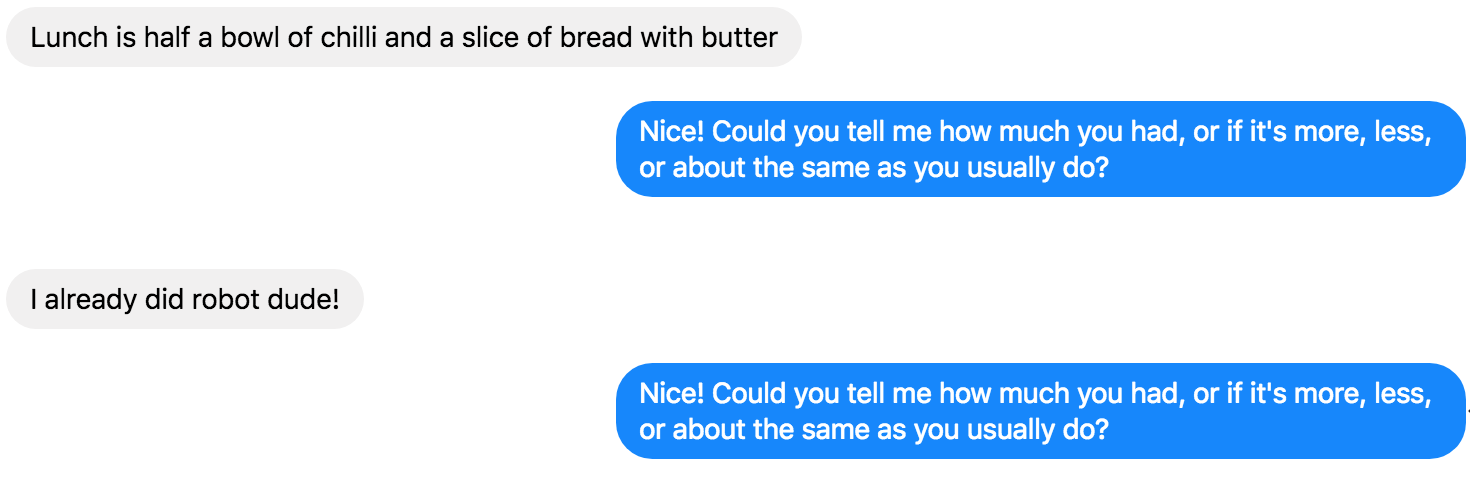
\includegraphics[width=\linewidth, height=6cm,keepaspectratio]{Nice2.png}
    %\caption{More coffee.}
  \end{subfigure}
\end{figure}
This also caused the intent recognition model to have several false positives, misidentifying stop words as food within a message that also contained valid food words. Fortunately, this kind of false positive turned out to be less relevant, because the user would already have to identify some portion sizes, so they would not notice misidentification issues, and the recognised food was only stored in the database if matching with some record in the \textit{Nutritionix} API. But while the API did provide a safeguard against incorrect food identification, it also showed issues by misidentifying real food, either by catching only part of the word (cupcake was flagged as cake mix in one instance), or sometime inexplicably (Long island ice teas were stored in the database more than once, without the user having logged them). The ability to list several different food items within a single message, as well as users' habit of splitting up different elements of the same meal between different messages, also caused difficulties in matching quantity to food, with Dialogflow's models simply not being advanced enough to catch the many subtleties of word ordering. This was another cause for the size clarification message to be presented after a quantity had already been given.\\
The \textit{clarifai} API rarely conformed to our ideal parameter of a single identification over the 97\% confidence threshold; however, the among the top three choices, there was often a good candidate the user could choose to select. When confronted with no suitable choice, if the user tried to clarify what the food was, the chatbot appeared to recover gracefully, while actually logging the clarification as a new meal. \\
A considerable effect on how the chatbot performed with users was also due to operational issues. After obtaining consent to participate in the experiment, users were provided with a URL they could open through the Facebook Messenger app or in the browser. Before it became clear that individual users had to be added as testers through the Facebook developer console, the first users who were given a URL did not receive any reply to their messages until they were added. While it was explained to them that this was not an issue with the chatbot but a temporary account management problem, it might have contributed to the perception that the chatbot was buggy. In fact, even after testing initiated correctly, there were some uncaught bugs that users could easily spot, which betray the fact that they were conversing with an automaton. For many of the chatbots' interactions, responses were selected randomly from a predefined list; over time, the user would exhaust all variants for a response, and since these were selected randomly sometimes would have the exact same responses given to them in quick succession. Sometimes, the database would fail silently when accessing the user name, so a message would be sent to the user containing ``undefined'' rather than their name. \\
Perhaps most grievously, an uncaught exception in the logic of \textit{worker.js} caused the entire periodic reminder script to fail after having sent messages to the first user. Because the first user was our test account, we kept receiving reminders through the evaluation period, which caused us to believe everything was behaving correctly until the 6th day of the experiment. Since this was a very important feature we were interested in evaluating, we decided to push a fix in production, and to extend the trial by two more days to verify its effects. We deactivated the reminder for feedback after 3 days had passed, because with the change in schedule it would have fallen too close to the conclusion.
The fix was not perfect, causing the no log reminder to fire up for every user, even if they had just logged their food the night before. However, while this might have been annoying for these users, it proved highly effective, causing every single user to log at least a meal on the day and after, including those who had only tested it on the first day and given up after. The leafy greens reminder was also subjected to a similar bug, firing for every user just before the no log reminder. Unlike the latter, most users did not seem to react to the suggestion, and while some registered the message, it is unclear whether users failed to modify their behaviours because the greens reminder encourages a more difficult change, or simply because they only noticed one of the remainders. The second explanation is not unlikely, given the fact that our testers seem to ignore larger body of text while messaging, like the introductory welcome message which explained the chatbot's capabilities, causing users who were not given an explanation before the experiment to be unaware of some functionality. \\
Another functionality that was not presented to the user due to some small logic errors was the under or overeating reports. One of the condition for undereating was that if only two small items of food were inserted before 11 PM, we should flag an undereating option; this however should only have applied if the request was made for food on the current day. causing previous days' requests executed before 11 not to trigger. This issue might however be considered negligible for the purposes of our evaluation, since users rarely asked for previous days' logs.
\section{Evaluation results}
While our study provides us with some interesting qualitative data, it should be noted that we cannot conduct hard generalisations on our results, because of the tiny sample size. Our participants come from the uniform demographic of university students because of issues with the logistics of recruitment; while this enables us to compare data without taking into account how demographics affect replies, it also means we lack external validity, and we cannot understand how other groups, especially in vulnerable less tech-savy age groups or with have major dietary issues, will react. Further studies will be necessary to ascertain how usable the interface is for different demographics. \\
Responses to our survey confirmed that the chatbot is not ready for public release, and in its current incarnation provides little utility compared to app based food diaries; however, under some metrics the chatbot did provide a stronger performance, leaving open the possibility that with more work it might provide a suitable replacement. \\
More than one participant did note that interacting with the food log through conversation was, despite the frustrations with some faulty NLP, a benefit over MyFitnessPal, even wishing that the conversations could be more human like. In fact, while more users rated MyFitnessPal as being useful compared to the chatbot, the chatbot was rated as more pleasant to use than the app, despite the bugs. \\
Some evidence that the chatbot interface is easier to interact with than the MyFitnessPal menu can be glimpsed from the fact that a higher proportion of users did not log their meals because they were too busy or it would have been too much of a hassle. Indeed, there were complaints about the speed of entering a meal into the app being too slow.\\
Conversational interfaces also seem to influence users' thoughts on how food should be measured in logs, with participants who were exposed to chat marking a preference for keeping measurement relative to previous meals, as opposed to MyFitnessPal users preferring absolute measurement. This can be attributed as a reflection on the functionality provided by the two systems: our chatbot does not provide precise calorie counting calculations, making it less important to have a precise metric on how much food has been eaten. This can make food logging easier, because the user does not need to worry about using a scale or counting portions, but only need to give the easy estimation on how much they have eaten compared to previous meals. Of course, having precise quantity would enable us to perfect data analysis on the backend, but having a relative measurement already allows us to build simple heuristics such as ours to detect any new over or undereating trend in the users' habits, and there are some research projects looking into using machine learning to supplement missing health data \cite{wolters}. \\
Conversational reminder seem to be more effective than regular app notifications: every user of the chatbot logged a meal after receiving a reminder, while MyFitnessPal users who had turned on reminders did not act on them, or reported that they probably would not have been convinced by a reminder to log food. This of course might have been caused by the sparsity of reminders, since we never sent any in the first few days of the trial, and reminders to take actions outside the chatbot, like eating some leafy green vegetables, were not acted on. Nonetheless, users seemed to react favourably to the feature, and even requested having more frequent notifications to avoid skipping further meal logs. \\
The most important outcome from the survey that we did not observe during the previous evaluation trial was the issue of feature discoverability. Our solution of simply stating the chatbot functionalities in the opening message did not work, causing a significant number of participants not to be aware of features like picture logging or past logs requests. Users also reported not knowing about the analytics function the chatbot had, but those were intentionally left vague in the welcoming dialogue. The onboarding information was presented as a rapid succession of messages, which were also longer than usual, and the combination might have proven too much for the users who just scanned their content quickly. We also provided a helper message in case someone needed reminders on how to use the bot, but it was never invoked. Potential solutions to this issue include improving the initial dialogue, making it more interactive, breaking down the onboarding into a more gradual set up over the first day, or, taking a page from what most current Facebook Messenger bots do, using a persistent menu, which somewhat nullifying the benefits of having a conversational interface, and always presenting all features as quick reply options at the end of a previous conversation. This approach is highly recommended, as it provides user with a visual list of all input possibilities, as well as giving the chatbot a good understanding of what the user is intending to do, effectively resolving issues such as our chatbot's tendency of misclassifying an excessive amount of messages as food insertions. While we had been aware of this approach during development, we chose not to use it because in our opinion it broke the suspension of disbelief of having a conversation with an intelligent agent; in retrospect, it would have greatly improved our design, and it would be easier for user than being explicitly \textit{trained} into using the correct formulation to match an intent. \\
Across both platform, we saw a common trend of users not being able to draw any utility from the logging because they considered themselves to already have a good grasp of their diet. As much as users may believe that is the case, the advantages for more conscious users will emerge through further data analytics over larger period of times to identify long term trends, and better visualisation tools to display more useful information. In the case of the chatbot, since textual feedback is somewhat limited in the type of information we can display to the user, it would be beneficial to insert a webview within the Messenger app, which could enable us to display rich graphical content (the Forksy chatbot has a nice graphical overview for a user's food diary). \\

\begin{figure}[h!]
  \centering
  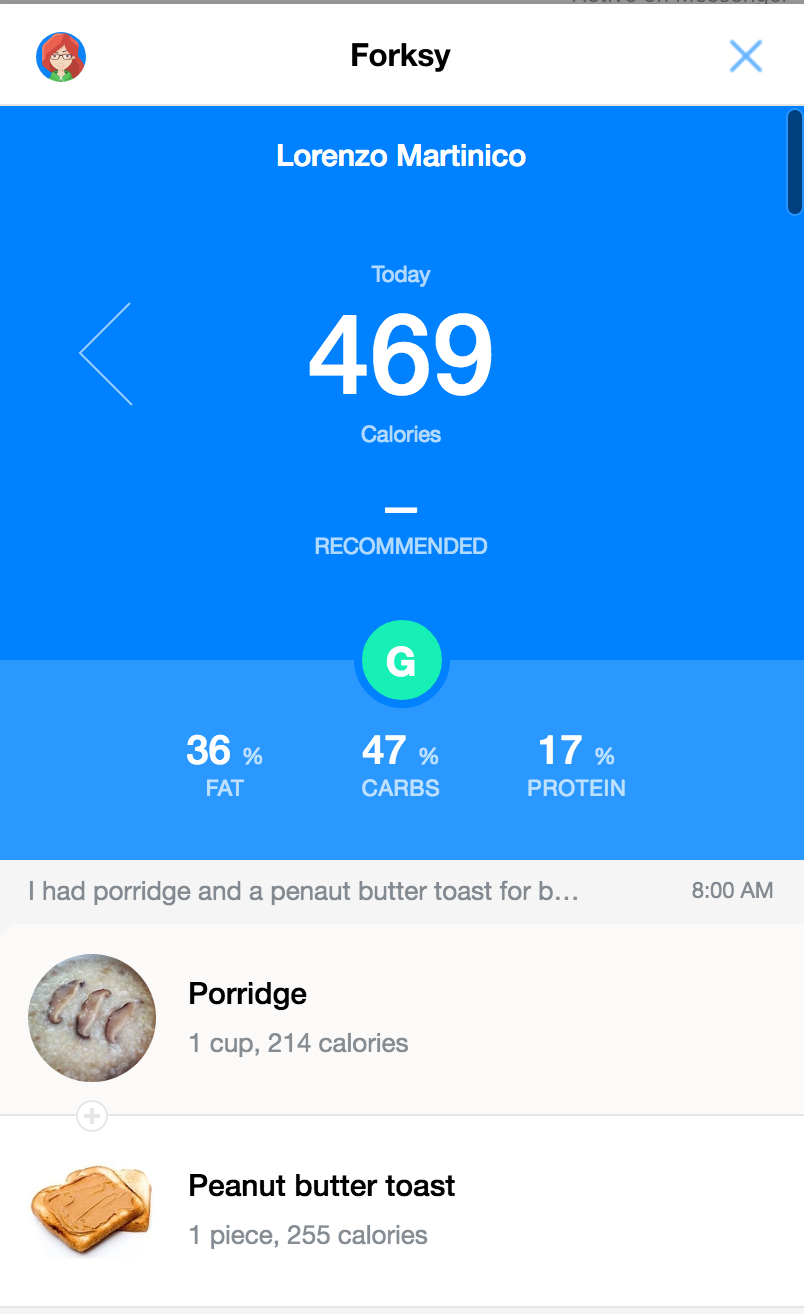
\includegraphics[height=14cm, keepaspectratio]{Forksydiary.png}
\end{figure} 

More adequate feedback could also be provided by taking into account users' goals and dietary preferences. It is meaningless to send a warning for having too little or too much food if we do not know whether the user is trying to lose weight or training to build muscle, and it might be harmful for users who already struggle with dieting to receive feedback their not having enough nutrients. Knowing whether a user is on a special diet, such as vegetarian or vegan, would also be beneficial, both for keeping track that users are getting all their nutrients, and to avoid making inappropriate recommendations for food that is missing from their diet. \\
Since our chatbot deals with people who may be in the vulnerable frame of mind of being insecure about their diet, we have to take extra care of what users are saying. Running some sentiment analysis on user input may avoid tragically inappropriate exchanges such as this, caused by the random selection of encouraging phrases in response to logging food, which besides making the user feel mocked also betrays our lack of understanding of the input's context. \\

\begin{figure}[h!]
  
\includegraphics[width=\linewidth, keepaspectratio]{Nice6.png}
\end{figure}

Some interesting feedback we received through the surveys was about user's mental model of how the chatbot worked (or rather, didn't). Users attributed undue relevance to the ``seen'' message icon on the Messenger application. While this would appear whenever a reply was sent, it would remain unmarked when the chatbot received a message it did not acknowledge it. The lack of read receipt co-occurred in some occasions where some expected remarks were not sent, most likely due to the Heroku server not waking up in time, causing users to associate the two events. Similarly, after the erroneous reminder for lack of usage was sent overnight, participants reported the chatbot not being able to distinguish whether they were sleeping or putting off logging food. These assumptions can be powerful to leverage when designing our conversations, by exploiting users' misconceptions to cover up flaws in the dialogue system. More studies should be conducted in this area. \\


\section{Future improvements} 
% maybe goes in conclusion?
There are many directions in which a project like this could go, and while our implementation was a bit barebones and only offered the essential features, there are several things we thought of during development or received requests from users which we might have added to make for a more useful and complete nutritional assistant, but had to hold off from because of time constraints. \\
An immediate feature addition that was reported as being useful during evaluation, was the option of retroactively adding a meal to the previous day. We immediately added the feature, which was a simple fix of changing the date object in the MongoDB update code from statically being the current date to taking the intent's argument. We did not push the new feature however because we were concerned deploying it would affect current users. \\
To match our functionality with MyFitnessPal's, we should also allow easy scanning of commercial food packages through a barcode scanner. While we could enable scanning on submitted images, this could lead to negative user experience when testing with badly framed images, requiring several photographs of the food to be taken before a match would be identified. Instead, we could rely on a Facebook Messenger webview object to integrate a live barcode scanner\footnote{possibly integrating https://github.com/serratus/quaggaJS}, but it is uncertain how well it would perform. \\
People interact in different ways with modern messaging platforms, and our chatbot should be able to take advantage of these new forms of communications: emojis, stickers, gifs. There are tagsets to classify this rich content based on emotion expressed, so we could use this as a basic form of sentiment analysis for incoming message, and to express personality when sending outgoing messages. We already have some hardcoded emojis as part of our script, but adding stickers and gifs to a generative model for text would make the chatbot feel more like a real entity, since the number of options is very large compared to the number of scripted responses we can write. \\
Some people tend to have a very regular diet, where they will eat the same meal for several days in a row. MyFitnessPal acknowledges this, and it provides an option to copy a meal from a previous day. This interaction pattern would fit naturally with a chatbot dialogue, where a user could simply say: ``I had the same breakfast as yesterday'', and the system should just replicate the same food as in the previous day. Of course, this would require enforcing a more strict separation between meals that we currently have, but we could guess it based on time of input, or by simply setting the meal type as a required parameter in the logging intent. Even simpler, although a bit less natural, would be asking the chatbot to set a recurring meal to be copied every day until manually interrupted. \\
A feature that was particularly appreciated by MyFitnessPal testers was recipe suggestions. It would be good if the chatbot could automatically suggest recipes, based on what nutritional requirements the user needs to fulfil, and maybe taking into account dietary history and preferences. In fact, with enough food data it might be possible to infer what kind of foods the user likes, and aggregating data across several users we might be able to provide a recommender system for discovering new recipes you might not know. \\
A nutritional assistant should also be able to give you some advice on specific food. It would be pretty simple to add an intent to query information from the \textit{Nutritionix} API about the nutritional values of the food in question. However, the challenging aspect of such a feature would be displaying the information in a useful way. It could be possible to display nutritional content in grams for each macro and important micronutrients, but that would only benefit people who can understand what those nutritional values mean, and does not fit within the final aims of our chatbot. Perhaps contextualisation with past meals might provide useful, but we need to be able to classify what kind of food that is, which is still an unknown problem.\\
We should also be interested in tracking other factors beside the food eaten. Sleep, mood, level of stress and exercise are all massive factors that can affect and be affected by what we eat \cite{buman2015physical}. The chatbot should capture these factors, either by interfacing with another quantified self platform, or by asking users questions at the start of the day. \\
The above features would mostly be relatively straightforward to implement, and we would have added them to our chatbot if we had had more development time available. We also envisioned several other possible features, which would be interesting, but would also require a lot more work to make possible. \\
An interesting component in diet tracking is social awareness, as discussed in the Background chapter. While the chatbot interface in itself does not provide any obvious advantage from this point of view, the network effect of having an agent that can interact with your contacts, be it your social circles in Facebook Messenger or your co-workers on Slack, can provide some interesting opportunities to leverage social pressure. The most immediate idea is having the chatbot set ``challenges'' to a group of users. This might take the form of a user invoking the chatbot in a group chat through the Facebook Chat Extensions \cite{chatextensions}, and setting a randomised ``healthy eating'' challenge (something along the lines of \textit{eat 5 portion of vegetables every day for the next week}). The chatbot would then end ask for participants among the group chat members, and once everyone has accepted or declined the challenge, it would keep a score of how everyone is doing, publicly complimenting those who are on track and encouraging who has been lagging off to do better. To avoid polluting the group chat, whose purpose might not be just having fitness challenges, logging should happen within the regular direct message interaction with the chatbot, and shoutouts and encouragements should be limited to a small daily window. \\
The idea of using the chatbot has a motivator tool to set challenges against themselves could also be expanded to the context of an individual user. This would work very similarly to the group challenges, except the user would be competing against themselves, trying to surpass their previous goals or stick with a new healthy habit. \\
We would also like to go back to our original idea of integrating images from social networks. With Instagram being impossible to use (besides scraping public facing profiles through a crawler), Flickr seems like the best alternative. Syncing with a user's photo collection allows us not only to save time from logging their new meals, and to capture a snapshot of historic data, but also leverage metadata that the social network makes available to us, such as image tags and the social graph of people interested in that picture. This would help strengthen the prediction for our food classification, but would also provide a basis to group related foods together. \\
Another helpful deception our chatbot could adapt, until an appropriate nutritional knowledge base and algorithms to understand an individual's diet can be developed, would be giving a trained nutritionist the possibility to examine data that has been submitted so far, and intervene to give appropriate advice. Facebook Messenger does expose a Handover protocol \cite{handoverfaceboo}, designed for such a case where a human operator needs to takeover the chatbot's operations. We would also need to have some visualization tool, so that the human nutritionist might understand at a glance what the situation is and offer the necessary advice.

\section{Chatbots and privacy}
Throughout our implementation and evaluation phases, it became evident how little privacy a chatbot user can expect. Participants on our experiment, who come from a variety of academic background, mostly showed having some expectations of privacy, regardless how much they were concerned about the confidentiality of this specific domain, and overall user across Europe report greater concerns with how their personal information is being handled \cite{europasurvey}. \\
In our architecture, we had several stages where data was ``leaked'' to a third party: all communications between users and chatbot were completely accessible to Facebook, as the provider of the Messenger platform, and us, as well as any other potentially malicious administrators to the Facebook page the bot was linked to; all conversations were also forwarded to Google, to be analysed as part of their Dialogflow service; food eaten was stored on our MongoDB provider website; and some logs were leaked to the Heroku instance from our webhook code, which potentially could have stored a lot more information than it did. All of this data was associated with a personal identifier, or even the user's own name. \\
While ideally we should be able to trust these service providers with user information, revelations in the last few months have increased user's awareness, and concerns, with certain data brokerage and collection practices that are common among the tech giants, which leave data vulnerable to be exploited by malicious agents. And while the sensitivity of nutritional habits may not seem important, up until you consider how major eating disorders might be considered by insurance companies, using a chatbot in any other medical setting might be a cause of concern. Narrow rules in the United States govern how medical sensitive informations can be dealt with (regulated by the Health Insurance Portability and Accountability Act), and soon Europe will enforce data protection on its citizens (through the General Data Protection Regulation). \\
While most of the major messaging platforms nowadays provide an option for end-to-end encryption, especially thanks to the Signal Messaging protocol \cite{signal}, which has been widely deployed through industry, no one provides facilities to encrypt chatbot conversations \cite{Alesanco2018}, except the Wire messaging app, which has a barebones chatbot API in alpha stage (but it is unclear whether it is actually being used beyond their initial demos \footnote{https://github.com/wireapp/wire}), and the Matrix protocol \footnote{https://github.com/matrix-org}, which allows chatbot users within encrypted channels, but does not provide an officially documented API to develop them, which means there are about a dozen customly developed bots available. While an API such as Wire's uses end-to-end encryption to protect messages from the platform provider, a user still has to trust the other end, whoever controls the server the chatbot runs on, not to steal their data or leak it to malicious third parties. It might be possible to mitigate this risk with a revised client-only chatbot architecture, where some basic parsing happens immediately on the client side, perhaps using historic chatbot technologies such as AIML \cite{aiml}, or some ondevice machine learning, which has become more feasible in the past few years. This architecture would still include a server, whose only function would be storing the encrypted data, and conduct the relevant data analytics in an anonymous and confidential manner by using zero-knowledge proofs, an encryption scheme which enables a system to prove properties of a message without decrypting it. Of course, this would probably prevent more complex natural language processing which requires large scale data analysis, but maybe with proper conversation design it could be enough to maintain all important functionality, and any necessary data collection to improve on-device machine learning models might be conducted through privacy preserving techniques.
% cite MFP hack!!
% elaborate on dealyed interval's effectiveness
\chapter{Conclusion}
The main goal of our project was creating an alternative interface to make it easier for health data to be collected and understood.

Our implementation had us explore the architecture of popular SaaS toolkit Dialogflow and its functionalities, working with a platform that has only been superficially documented to create a fully functioning agent. We evaluated some basic principles of chatbot dialogue design, various back end technologies to finally choose Heroku, an option that would grant us the most flexibility and ease of use. We also explored the space of various third party tools, such as database technologies, nutritional information databases, image recognition for food objects and social networking APIs. While our original design included a vast breadth of features, having to deal with time limitations forced us to take into consideration what aspects of the interface would be truly fundamental, and prioritise what would take us to a minimum viable products. We highlighted some issues we ran into along the way, from failing to obtain permission to use the Instagram API for our purposes, to collecting a sufficiently large dataset of food names. Particular effort was put into classifying food based on its nutritional value, but we failed to achieve even barely usable performance, due to the complexity of the problem domain.

Despite the many roadblocks, we delivered a functioning prototype, the first chatbot, to our knowledge, which combines texting and pictures as input for a dietary log. We also led the first comparative user trial between a food logging app and chatbot, with a small group of tester across a single demographic. \\
While our final release was still plagued by many bugs that affected usability, we were able to provide a useful service to some users who gained some insights into their diet. Comparing our chatbot testers with the control group, we even achieved better results than MyFitnessPal in some areas, such as reminders and general pleasantness of use, and found out some interesting correlations between platform used and importance attributed to measurement units, as well as users' mental models and attitudes towards the confidentiality of nutritional data. 

This leaves us with some promising expectations for future progress of the project, and we explored some possible extensions of various implementation difficulties. Although these features might improve how much users can do with our chatbot, and how it feels to interact with it, we will still have to find a definitive way to replace our ad-hoc heuristic with a fully scalable and complete knowledge base, which would require a more systematic approach in its design, as well as larger scale testing. \\
As widely as these areas could be explored in the next phase of our project, however, during development, and from feedback we received in our evaluation, we realised that it would be impossible to create a chatbot that deals with medical data without compromising user's trust. Therefore, we would like to redirect our enquiries into exploring the possibility of having a secure chatbot, either from an architectural point of view, or in relation to their compliance with the upcoming General Data Protection Regulation in Europe. We realise that seems to go against recent trends in industry, where increasing data collection to enable intelligent features has become the norm; but the ever increasing hacks and information leaks, including from two of the service providers in our evaluation, and concerns for government and corporate surveillance keep reminding us how important privacy is. We recognise that chatbots can create an illusion of intimacy that might lead to sensitive information being shared more willingly, and because users have a right to have their most personal data protected, it is necessary to create a solution that will offer all advantages of conversational interfaces in a trusted and secure manner.


% use the following and \cite{} as above if you use BibTeX
% otherwise generate bibtem entries
% consider \nocite{*}
\bibliographystyle{plainurl}
\bibliography{bibliography.bib}

\end{document}
